\begin{center}
\begin{minipage}{0.49\textwidth}
\begin{center}
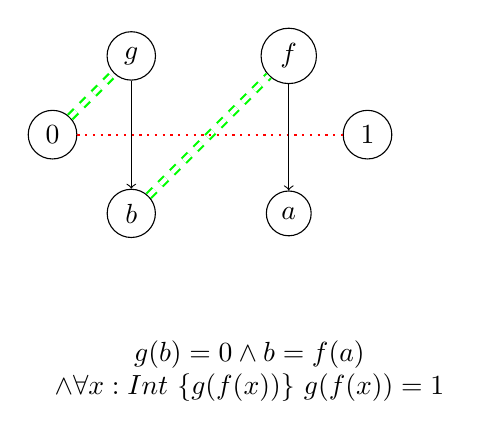
\begin{tikzpicture}
\node (b) [draw, circle, minimum size=0.8, align=center] at (0,0) {$b$};
\node (a) [draw, circle, minimum size=0.8, align=center] at (2,0) {$a$};
\node (g) [draw, circle, minimum size=0.8, align=center] at (0,2) {$g$};
\node (f) [draw, circle, minimum size=0.8, align=center] at (2,2) {$f$};
\node (0) [draw, circle, minimum size=0.8, align=center] at (-1,1) {$0$};
\node (1) [draw, circle, minimum size=0.8, align=center] at (3,1) {$1$};

\draw [double, dashed, thick, green, double distance=1.5] (0) -- (g);
\draw [double, dashed, thick, green, double distance=1.5] (b) -- (f);
\draw [red, dotted, thick] (0) -- (1);

\draw [->] (g) -- (b);
\draw [->] (f) -- (a);

\node [align=center] at (1.5,-2) {$g(b)=0 \land b=f(a)$\\ $\land \forall x:Int\ \{g(f(x))\}\ g(f(x))=1$};
\end{tikzpicture}
\end{center}
\end{minipage}
\begin{minipage}{0.49\textwidth}
\begin{center}
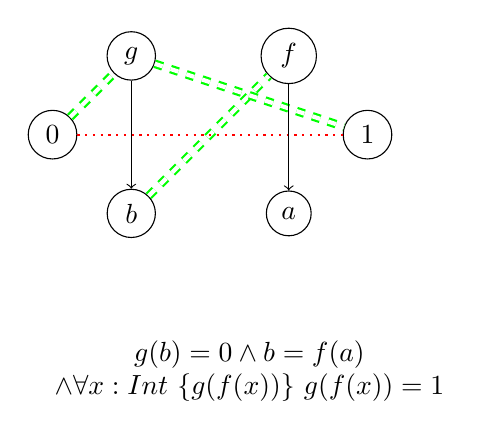
\begin{tikzpicture}
\node (b) [draw, circle, minimum size=0.8, align=center] at (0,0) {$b$};
\node (a) [draw, circle, minimum size=0.8, align=center] at (2,0) {$a$};
\node (g) [draw, circle, minimum size=0.8, align=center] at (0,2) {$g$};
\node (f) [draw, circle, minimum size=0.8, align=center] at (2,2) {$f$};
\node (0) [draw, circle, minimum size=0.8, align=center] at (-1,1) {$0$};
\node (1) [draw, circle, minimum size=0.8, align=center] at (3,1) {$1$};

\draw [double, dashed, thick, green, double distance=1.5] (0) -- (g);
\draw [double, dashed, thick, green, double distance=1.5] (b) -- (f);
\draw [double, dashed, thick, green, double distance=1.5] (g) -- (1);
\draw [red, dotted, thick] (0) -- (1);

\draw [->] (g) -- (b);
\draw [->] (f) -- (a);

\node [align=center] at (1.5,-2) {$g(b)=0 \land b=f(a)$\\ $\land \forall x:Int\ \{g(f(x))\}\ g(f(x))=1$};
\end{tikzpicture}
\end{center}
\end{minipage}
\captionof{figure}{E-graph before and after E-matching}
\end{center}